\documentclass[11pt]{article}
\usepackage[english, czech]{babel}
\usepackage[a4paper, top=3cm, left=2cm, textwidth=17cm, textheight=24cm]{geometry}
\usepackage{fontspec}
\setmainfont{Times New Roman}

\usepackage{environ}
\NewEnviron{centerbox}[1][\linewidth]{% \begin{centerbox}[..] ... \end{centerbox}
  \noindent\makebox[\linewidth][c]{%
    \begin{minipage}{#1}%
      \raggedright% Minipage alignment
      \noindent\BODY% Typeset body/contents
    \end{minipage}%
  }
}%

\usepackage{parskip}
\usepackage{amsmath}
\usepackage{rotating}
\usepackage{tikz}
\usepackage{multicol}
\usepackage{wrapfig}
\usepackage{graphics}
\usetikzlibrary{arrows,automata}
\usepackage{pdflscape}

\usepackage{csquotes}
\usepackage[unicode,pdftitle={Překladač pro jazyk IFJ20},hidelinks]{hyperref}
\usepackage[backend=biber,style=iso-numeric,autolang=other,sortlocale=cs_CZ,bibencoding=UTF8,block=ragged]{biblatex}
\addbibresource{bibliography.bib}

\usepackage{array,etoolbox}
\preto\tabular{\setcounter{rule_table_number}{0}}
\newcounter{rule_table_number}
\newcommand\rownumber{\stepcounter{rule_table_number}\arabic{rule_table_number}}

\begin{document}

\begin{titlepage}
	\centering
	
\includegraphics[width=\textwidth]{img/FIT_barevne_CMYK_CZ.pdf}
	\par
	\vspace{\stretch{0.382}}
	
	{\huge\bfseries Překladač pro jazyk IFJ20 \par}
	{\Large \textbf{Dokumentace k projektu} \par}
	{\Large Tým 056, varianta II \par}
	\vspace{2cm}
	
	\Large{
	\begin{tabular}{r l | r}
	    František Nečas (xnecas27) & & 33 \% \\
	    Ondřej Ondryáš (xondry02) & & 33 \% \\
	    David Chocholatý (xchoch08) & – vedoucí & 34 \% \\
	\end{tabular}
	}
	
	\vspace{2cm}
	
	{\Large Podporovaná rozšíření: \par}
	{\large BOOLTHEN, BASE, FUNEXP, MULTIVAL, UNARY \par}
    
    \vspace{\stretch{0.618}}

	{\large \today\par}
\end{titlepage}

\tableofcontents
\newpage

\section{Práce v týmu}

Časový rozvrh práce jsme si naplánovali už při návrhu překladače a~v~průběhu implementace pouze mírně upravovali podle nutnosti. Termíny se nám dařilo dodržet, přestože jsme v~závěru lehce zaostávali oproti původnímu plánu, měli jsme připravenou dostatečnou rezervu na pokrytí těchto výchylek od plánu.

Práci jsme si rozdělili již v~začátcích, často jsme však spolupracovali při implementaci rozhraní mezi moduly a~diskutovali způsob jejich vzájemné komunikace, případně praktikovali techniku párového programování (například ve finální fázi propojení jednotlivých částí překladače).

\subsection{Rozdělení práce}

\begin{itemize}
	\item David Chocholatý (xchoch08)
	    \begin{itemize}
	        \item scanner, chybové zprávy na stderr, integrační testy překladače, LL(1) gramatika, Makefile, code review, hashovací tabulka, dokumentace
	    \end{itemize}
	\item František Nečas (xnecas27) 
	    \begin{itemize}
	        \item syntaktická analýza (rekurzivní sestup a~precedenční SA), základní sémantické kontroly, optimalizace kódu, tvorba vnitřní reprezentace, implementace dynamického řetězce, code review, automatické Travis testy, dokumentace
	    \end{itemize}
	\item Ondřej Ondryáš (xondry02)
	    \begin{itemize}
	        \item kostra pro testování, testy pro scanner a~parser, datové struktury pro vnitřní reprezentaci kódu (\emph{control flow graph} a~\emph{abstract syntax tree}), Makefile, generátor cílového kódu, code review, dokumentace
	    \end{itemize}
\end{itemize}

\subsection{Organizace práce}

Při vývoji byl použit verzovací systém Git, členové týmu pracovali ve vlastních vývojových větvích a před začleněním nového kódu do hlavní větve byl vyžadován pull request, code review a schválení od ostatních členů týmu. S repozitářem byl spojen také systém \emph{průběžné integrace} Travis CI, který na nových commitech automaticky spouštěl jednotkové a integrační testy, které jsme psali v C++ s použitím testovacího frameworku Google Test. Komunikační platformou týmu byl Discord.

\section{Návrh překladače}

Náš překladač stojí na syntaxí řízeném překladu provádějícím jednoprůchodovou analýzu zdrojového kódu. Jednoprůchodovou analýzu jsme zvolili, protože program je čten ze standardního vstupu a~pro dvouprůchodovou analýzu by bylo třeba neefektivně ukládat celý řetězec tokenů. Vytváří si vnitřní kód v~podobě abstraktních syntaktických stromů. Na úrovni vnitřní reprezentace provádí různé optimalizace kódu. V~případě nalezení chyby v~překládaném kódu je schopen se z~chyby zotavit a~pokračovat v~kontrolách nadále, ovšem již bez generace cílového kódu.

\subsection{Scanner}
\label{scanner}

Scanner implementujeme jako deterministický konečný automat. V~\hyperref[sec:fa]{příloze} \ref{sec:fa} lze nalézt diagram tohoto deterministického konečného automatu.

Scanner je volán parserem, který scanneru předá informaci o~EOL pravidlu vyžadovaném pro následující token (\emph{required}, \emph{forbidden}, \emph{optional}). Dokud scanner nenačte první znak nového tokenu, testuje, zda kód toto pravidlo splňuje. V~případě chyby vrací parseru prázdný token s~chybovým návratovým kódem podle typu chyby. Scanner tedy pracuje s~EOL jako s~bílým znakem, u~kterého si ale poznačí, že byl přečten, a~vyhodnotí podle požadovaného pravidla případnou chybu.

Scanner vrací parseru načtený token s~atributy souvisejícími s~daným tokenem \footnote{typ tokenu, pro čísla a~boolean odpovídající hodnoty, dynamický řetězec pro identifikátory a~řetězce} a~rozšířeným kontextem tokenu s~informací o~čísle řádku a~sloupce v~kódu (pro výpis chybových hlášek) a~případně informací o~přečtení znaku nového řádku.

Scanner také rozhoduje, zda se v~případě načteného identifikátoru nejedná o~klíčové slovo. Tehdy uvolní načtený řetězec a~vrací token identifikátoru s~atributem informujícím o~typu klíčového slova.

Ke komentářům se scanner chová jako k~bílým znaků za předpokladu, že jsou korektně zapsány \footnote{IFJ20 nepodporuje například vnořené blokové komentáře aj.}. Pouze v~tomto případě odliší EOL znak od jiných bílých znaků, aby mohl ověřit korektní ukončení řádkového komentáře. Obsah komentářů se zahazuje, nepracuje se s~ním.

Pro kontrolu lexikálních chyb a možnost vypsání lepší chybové zprávy se scanner může podívat na následující znak, který v~případě, že se nejedná o~část současného tokenu, uchová v~paměti pro~pozdější volání scanneru. Pokud se jedná o~chybu, ale konečný automat se nachází v~koncovém stavu, scanner vrací tento token a~chybu zahlásí až při jeho dalším volání, kdy začne číst od předem načteného znaku, který ale automat nepřijme.

V~případě načtení EOF se scanner pokusí dokončit aktuálně čtený token a~vrátí tento token spolu s~informací o~přečtení celého zdrojového souboru.

\subsubsection{Dynamický řetězec}
Pokud si scanner potřebuje ukládat čtené znaky\footnote{K~tomu dochází při načítání znaků identifikátoru, řetězce nebo čísla}, použije abstraktní datový typ \emph{mutable\_string}, který je implementován jako nafukovací pole. Umožňuje vkládat po znaku do už existujícího řetězce a~řeší konkatenaci dvou řetězců. Také je předáván v~tokenu parseru pro identifikátory a~řetězce.

\subsection{Parser}

Parser jsme implementovali pomocí metody rekurzivního sestupu založené na LL(1) gramatice a~pomocí precedenční syntaktické analýzy pro výrazy.

\subsubsection{Rekurzivní sestup}

Při implementaci rekurzivního sestupu jsme se inspirovali jednoduchým interpretem zveřejněným na stránkách IFJ. Jak již bylo naznačeno v~sekci \ref{scanner}, v~našem překladači nevytváříme token pro znak nového řádku a~do gramatiky tedy tento terminál neuvádíme. Při volání scanneru jsme nastavovali příznak pravidla nového řádku na základě specifikace v~zadání a~kompatibility s~jazykem Go. Tím ovšem vzniká problém v~\hyperref[sec:ll-tab]{LL tabulce}, kdy po klíčovém slovu \texttt{return} může následovat výraz ve dvou různých významech, jako návratová hodnota, nebo jako nový příkaz. Tento problém v~rámci implementace řešíme voláním scanneru s~příznakem \textit{optional} a~následnou kontrolou kontextu. Pokud nebyl znak nového řádku načten, patří výraz ke klíčovému slovu \texttt{return}, jinak se jedná o~nový příkaz.

Z~důvodu kombinace rozšíření MULTIVAL a~FUNEXP jsme se rozhodli zpracovávat i~příkaz přiřazení a~definice v~rámci precedenční syntaktické analýzy. Díky tomu je jednodušší provádět sémantické kontroly a~generovat vnitřní kód (v~jednom kroku je redukována celá definice, resp. přiřazení). Předání řízení tedy probíhá, když je očekáván výraz (například za klíčovým slovem \texttt{if}) nebo v~případě zpracování příkazu (zde ovšem musí výraz začínat identifikátorem, protože může následovat definice, přiřazení, nebo volání funkce). Problémem zde avšak je, že Go je velice striktní a~značně omezuje možnosti výrazů, není možné například řetězit operátory přiřazení, v~rámci cyklu \texttt{for} je vynucena definice a~přiřazení v~první, resp. třetí části. Dále také nejsou povoleny příkazy bez efektu. Proto rekurzivní sestup předává precedenční syntaktické analýze příznak specifikující, jaká jsou v~současnosti pravidla pro definice a~přiřazení.

\subsubsection{Precedenční syntaktická analýza}
\label{precedence}

Pro precedenční syntaktickou analýzu jsme implementovali zásobník přijímající nadmnožinu tokenů (načtený token je nakopírován do nové struktury a~doplněn o~další informace, například ukazatel na příslušný uzel abstraktního syntaktického stromu, viz \ref{sec:ast}). Tento zásobník je implementován pomocí obousměrně vázaného seznamu, aby bylo možné se v něm lehce pohybovat při hledání vhodného redukčního pravidla. Navíc poskytuje rozhraní pro nalezení vrchního neterminálu a~odstranění části obsahu od specifikovaného uzlu.

Konec výrazu je určen na základě příchozích tokenů a~načítání znaku nového řádku. Snažíme se zde co nejvíce držet kompatibilitu s~Go a~tedy za operátory, levou závorkou a~čárkou je povolen znak konce nového řádku. V jiných případech (například konec řádku po identifikátoru) se jedná o konec výrazu.

Při načtení identifikátoru je třeba určit, zda se jedná o~identifikátor proměnné, nebo funkce. Za tímto účelem jsme implementovali abstrakci nad scannerem, která umožňuje pouze nahlédnout na následující token (tento token se uloží do paměti a~při dalším volání této funkce je opět vrácen). Při načtení identifikátoru tedy parser nahlédne na následující token a~pokud se jedná o~levou závorku, považujeme identifikátor za funkci.

Aby precedenční syntaktická analýza mohla určit splnění platnosti příznaku předávaného rekurzivním sestupem, musí počítat některé parametry výrazu, konkrétně počet volání funkcí, počet definic, počet přiřazení a~počet ostatních tokenů. Na základě toho průběžně rozhoduje, zda nebyl porušen nastavený příznak, a~v~případě, že porušen byl, jedná se o~syntaktickou chybu. Po dokončení zpracování výrazu je rekurzivnímu sestupu předán odkaz na vytvořený AST a~informace, zda výraz byl platný.

\subsubsection{Sémantické kontroly}

Jednoprůchodová analýza omezuje možnosti provádění sémantických kontrol při zpracovávání výrazů. Kvůli rozšíření FUNEXP nemusí být možné odvodit ani typy argumentů při volání funkce (například při zanoření několika funkcí, které ještě nebyly definovány) a~je potřeba správnost volání ověřit až později. V~rámci parseru se tedy sémantická analýza snaží zkontrolovat vše, co je možné, tedy například kontroluje typovou správnost ve výrazech bez funkcí a~spekulativně vytváří položky v~tabulce symbolů pro funkce. O~typovou kontrolu funkcí se poté stará mechanismus typové inference AST (viz \ref{sec:inference}), který je spuštěn až ve chvíli, kdy už jsou načteny všechny definice funkcí, a~tedy dokáže ověřit úplnou správnost všech výrazů.

\subsubsection{Zotavení z chyb}

V rámci syntaktické analýzy jsme implementovali zotavení z~chyb na základě pevných klíčů. Jako pevný klíč v~tomto případě slouží znak nového řádku, který v~IFJ20 odděluje jednotlivé příkazy. Při nalezení chyby je volán lexikální analyzátor, dokud nenarazí na znak nového řádku (to je detekováno dle kontextu předaného spolu s~tokenem). Následně je znovu spuštěna syntaktická analýza od neterminálu \textit{body}, který reprezentuje jednotlivé příkazy v~těle funkce. Tentokrát už se ovšem nevykonávají sémantické kontroly a~končí generování vnitřního kódu, což je zajištěno pomocí nastavení globálního chybového stavu překladače.

\subsection{Vnitřní reprezentace kódu}

V rámci syntaxí řízeného překladu vytváří parser při své činnosti vnitřní reprezentaci kompilovaného kódu. Pro tuto reprezentaci jsme zvolili formu abstraktního syntaktického stromu. Ten je navíc rozdělen na dvě části: graf řízení toku\footnote{Ačkoliv jde také o~orientovaný acyklický graf, pro CFG nepoužíváme označení „strom“, protože má převážně lineární povahu a~nevyužíváme u něj vlastnosti stromů. Rozlišujeme u~něj ale kořenový vrchol.} (\emph{control flow graph}, dále pod zkratkou \emph{CFG}) a~samotné abstraktní syntaktické stromy (\emph{abstract syntax trees}, dále \emph{AST}). Toto rozdělení přirozeně vychází z~koncepce rozdělení syntaktické analýzy: CFG celkově popisuje strukturu programu -- definované funkce a~postup příkazů v~jejich tělech; v~rámci programu tvoří jediný celek a~je vytvářen při rekurzivním sestupu. AST je oproti tomu struktura, která popisuje zvlášť každý samostatný výraz (včetně definice či přiřazení) a~představuje tak samotné výpočetní kroky jednotlivých příkazů. AST je výstupem každého úspěšného průchodu precedenčním syntaktickým analyzátorem.

\subsubsection{Abstraktní syntaktické stromy}
\label{sec:ast}

AST je datová struktura tvořená výhradně vzájemně propojenými instancemi struktury \texttt{ASTNode}. Koncepčně se jedná o~binární strom: každý uzel obsahuje odkaz na otcovský uzel a~odkazy na levého a~pravého syna. Využívá se ovšem i~speciální typ uzlu \texttt{AST\_LIST}, který ve své datové části obsahuje libovolný počet ukazatelů na další AST uzly, přičemž nemá levého a~pravého syna. Tento typ uzlu se využívá pro definice, přiřazení a~návratové hodnoty (viz dále). Každý uzel může nabývat neomezené množství dat\footnote{s~využitím flexible array member na konci struktury}, daty je konstanta (číselná, řetězcová nebo logická), ukazatel na položku tabulky symbolů nebo ukazatel na jiný \texttt{ASTNode}. V~případě, že obsahuje data, se vždy jedná o~uzel listový.

Uzel AST může nabývat různých typů: Na konkrétní hodnotu vždy vedou uzly \emph{s aritmetickou operací}, uzly \emph{s logickou operací}, uzly typu \emph{konstanta} a~uzly typu \emph{identifikátor} (v~případě identifikátorů funkcí může jít o~hodnotu typu \texttt{\textit{NIL}} nebo \texttt{\textit{MULTIPLE}}, které nejsou použitelné ve výrazech); na hodnotu také může vést uzel \emph{volání funkce}, který dědí typ hodnoty svého identifikátoru. Naopak na hodnotu nikdy nevedou uzly typu \emph{definice} a~\emph{přiřazení}.

Jednotlivé typy uzlů mohou být přítomny jen ve specifických kontextech -- například příkaz CFG (viz dále) musí jako kořenový uzel AST obsahovat AST typu definice, přiřazení nebo volání funkce; příkaz větvení IF musí jako kořenový uzel AST s~podmínkou obsahovat AST, který vede na logickou hodnotu. Implementované kontroly těchto omezení jsou do jisté míry redundantní: například kód \texttt{if a := 5 \{} by neprošel už přes syntaktickou analýzu kvůli neexistujícímu pravidlu gramatiky, naopak v~případě \texttt{if 5 + 5 \{} už je kontrola na úrovni CFG/AST nutná. Různé kontroly typů uzlů a~datových typů (viz dále) implementované v~CFG/AST tvoří podstatnou část sémantických kontrol překladače.

\subsubsection{Inference datových typů}
\label{sec:inference}

Kvůli podpoře volání funkcí ve výrazech v~rámci rozšíření FUNEXP pro zajištění správného stromu nestačí pouze informace o~druhu AST uzlu, každý uzel musí být označen také datovým typem hodnoty, kterou po vyhodnocení představuje. Z~tohoto důvodu je v~rámci AST implementována \emph{inference datových typů}. Jedná se o~mechanismus, který rekurzivně prochází daným AST (průchodem typu post-order) a~podle zjištěných typů synovských uzlů nastaví typ zjišťovaného uzlu nebo zahlásí chybu. Algoritmus musí zároveň počítat s~případy, kdy v~danou chvíli není znám typ proměnné (například při definici) nebo návratové hodnoty volané funkce (pokud je v~kódu definovaná až později). Inference je totiž spouštěna pro jednotlivé AST poprvé při redukcích v precedenční syntaktické analýze, v~tu chvíli ještě informace o~typech nemusí být známy. Podruhé se inference spouští při optimalizaci některých výrazů, potřetí při generování kódu, a~to ve striktním módu, který ve většině případů nedovoluje AST uzly s~neznámým typem. To v~podstatě supluje roli druhého průchodu syntaktického analyzátoru.

V původním návrhu měla inference v~rámci AST poněkud menší význam, usoudili jsme ale, že nemá smysl provádět složitější typové kontroly v~rámci syntaktické analýzy samotné, když je (právě kvůli možnosti neznámého typu návratové hodnoty funkce ve výrazu) bude později potřeba provádět znovu v~jiné části kompilátoru\footnote{Pozůstatkem po původním návrhu je existence vnitřního chybového stavu AST, který se ale při většině kontrol nenastavuje, protože AST při chybě nyní přímo vypisuje chybovou hlášku a~nastavuje globální chybový kód kompilátoru.}. Do mechanismu inference typů jsme tak zařadili také sémantické kontroly volání funkcí (kontroluje, jestli při volání odpovídají počet a~typy argumentů) a~přiřazení (kontroluje, jestli je do už definovaných proměnných přiřazován správný typ, také umožňuje hromadné přiřazování více návratových hodnot funkce do seznamu proměnných). Typová kontrola také ukládá informaci o~zjištěném typu do tabulky symbolů.

Systém typové inference je vcelku mocný a~je schopen odhalit velké množství sémantických chyb, nutno ale podotknout, že naše implementace není příliš efektivní. Kvůli některým krokům, které nastávají při zjišťování typů u~volání funkcí, není možné spolehlivě vynechat inferenci ani pro uzly, které už typ přiřazený mají. Abychom mohli efektivně odhalovat sémantické chyby co nejdřív od jejich načtení parserem, voláme ji pro každý uzel na několika místech, proto se pro většinu uzlů volá inference několikrát a~mnohdy redundantně.

\subsubsection{Graf řízení toku}

CFG je grafová datová struktura s~několika druhy vrcholů, které mají svá specifika. \emph{Kořenovým} vrcholem je jedna instance struktury \texttt{CFProgram}, která v~sobě obsahuje obousměrně vázaný lineární seznam struktur \texttt{CFFunction}, které popisují jednotlivé funkce zdrojového programu. Tyto struktury dále obsahují obousměrně vázané lineární seznamy struktur \texttt{CFVariable}, které reprezentují argumenty a~návratové hodnoty dané funkce, a~ukazatel na první vrchol typu \texttt{CFStatement} představující první \emph{příkaz} funkce.

\emph{Příkaz} se zjednodušeně dá interpretovat jako popis jednoho řádku zdrojového programu. Příkazem může obecně být definice proměnných, přiřazení do proměnných, volání funkce, větvení, cyklus nebo návrat z~funkce. V~CFG je příkaz reprezentován strukturou \texttt{CFStatement}, která má jeden ze čtyř typů:
\begin{itemize}
    \item \texttt{BASIC}: Obsahuje přímo odkaz na kořen AST typu definice, přiřazení nebo volání funkce.
    \item \texttt{IF}: Obsahuje odkaz na kořen AST s~logickou hodnotou, který představuje podmínku větvení, a~odkazy na první příkaz (strukturu \texttt{CFStatement}) větve \emph{then} a~případně na první příkaz větve \emph{else}.
    \item \texttt{FOR}: Může obsahovat odkaz na kořen AST typu definice, kořen AST s~logickou hodnotou, který představuje podmínku pokračování cyklu, a~kořen AST typu přiřazení. Obsahuje odkaz na první příkaz těla cyklu.
    \item \texttt{RETURN}: Obsahuje přímo odkaz na kořen AST typu seznam AST; AST v~tomto seznamu reprezentují jednotlivé výrazy, které se vyhodnocují jako návratové hodnoty funkce.
\end{itemize}

Vrcholy \texttt{CFStatement} tvoří orientovaný graf -- na nejvyšší úrovni se dá také chápat jako obousměrně lineární seznam, příkazy typu IF a~FOR ovšem kromě předchůdce a~následníka obsahují také ukazatele na další větve. Vrcholy obsahují také další informace, zejména však ukazatel na tabulku symbolů, která k~danému příkazu přísluší.

CFG je implementován jako stavový modul, do kterého jsou pomocí rozhraní postupně přidávány jednotlivé vrcholy. Modul drží informaci o~aktuálně aktivním vrcholu, se kterým ostatní funkce v~daný moment operují. Způsob, jakým se mezi sebou vážou jednotlivé vrcholy, je pro zbytek překladače transparentní\footnote{Podobně byl v~prvotním návrhu implementován i~AST, při analýze zdola nahoru to však není praktické, proto finální implementace AST pouze usnadňuje vytváření uzlů a~jejich vázání do stromu zajišťuje přímo syntaktický analyzátor.}. Tento způsob implementace byl zvolen pro jednoduchou interoperabilitu se syntaktickým analyzátorem, který může jako sémantické akce při expanzích jednoduše volat příslušné funkce CFG.

\subsection{Optimalizátor vnitřní reprezentace}
Využili jsme tři optimalizační techniky nad vnitřním kódem. Nejdříve se volá skládání konstant a~propagace konstant, protože tyto akce se mohou vzájemně ovlivňovat. Tyto optimalizace se opakovaně spouštějí, dokud probíhají nějaké změny ve vnitřním kódu. Po dokončení se spustí odstranění mrtvého kódu.

\subsection{Skládání konstant}
Základní optimalizací našeho kompilátoru je vyhodnocování konstantních podvýrazů při překladu. Při této optimalizaci provádíme post-order průchod AST a~v~případě, že všechny operandy některé operace jsou konstantní, provede se zjednodušení AST. Dále také využíváme algebraických vlastností operací, například je tedy odstraněno přičítání nebo odčítání nuly, dvojitá negace (logická i~aritmetická) a~také je kontrolováno dělení nulou, což umožňuje pokročilou detekci této sémantické chyby.

\subsection{Propagace konstant}
V~rámci každé funkce se snaží optimalizátor nahradit ve výrazech proměnné, pokud do nich předtím byla pouze přiřazena konstanta, za tuto konstantní hodnotu\cite{ConstantPropagation}. Při průchodu funkce se do vázaného seznamu ukládají proměnné, které byly při definici inicializovány konstantou. Pokud je ovšem do proměnné přiřazen později v~kódu nekonstantní výraz, je třeba ji ze seznamu odstranit. Následně nad všemi výrazy probíhá post-order průchod a~v~případě identifikátorů se na základě ukazatele do tabulky symbolů a~seznamu proměnných s~konstantní hodnotou vyhodnocuje, zda může být nahrazen za konstantu. Problematické zde jsou cykly, kdy před propagací konstant do cyklu je nejdříve třeba ze seznamu konstant odstranit všechny proměnné, do kterých je v~rámci cyklu přiřazeno (ať už v~hlavičce cyklu, nebo v~jeho těle).

\subsubsection{Odstranění mrtvého kódu}
Po optimalizaci výrazů mohou vzniknout bloky kódu, které nikdy nebudou interpretovány. Takové bloky vznikají při větvení, kde může být po optimalizaci vyhodnoceno, že podmínka větvení bude vždy pravdivá či nepravdivá. V případě, že je podmínka cyklu for konstantně nepravdivá, je možné celý cyklus odstranit. Obdobně je možné odstranit nepravdivou podmínku if, ovšem zde převádíme \texttt{else} blok na příkaz typu \texttt{if true}\footnote{Takový blok by mohl být dále zjednodušen a~vložen přímo mezi sekvenci příkazů rodičovského bloku, to ale aktuální implementace nepodporuje.}. V~případě příkazu \texttt{if true} je možné odstranit \texttt{else} blok, protože se nikdy nevykoná.

\subsection{Generátor cílového kódu}

Generátor cílového kódu prochází v~CFG uložený lineární seznam položek \texttt{CFFunction} a~pro každou funkci spouští rekurzivní průchod jeho CFG. Při něm se postupně vyhodnocují jednotlivé AST a~výsledky vyhodnocování jsou přiřazovány do proměnných. V~průběhu syntaktické analýzy jsou u~symbolů nastavovány čítače užití, generátor tak může vypouštět definice proměnných, do kterých je pouze zapisováno.

\subsubsection{Konvence volání funkcí a~využití rámců}
\label{sec:konvence_volani}

\emph{Volající} vytváří dočasný rámec, ve kterém definuje proměnné odpovídající argumentům volané funkce. Tyto proměnné naplní vyhodnocenými hodnotami a~skočí na návěští funkce. Ihned za návěštím je dočasný rámec přesunut na vrchol zásobníku rámců, stane se tedy jejím lokálním rámcem. V~tomto rámci se následně manipuluje se všemi proměnnými funkce, žádné další rámce nejsou vytvářeny\footnote{Výjimkou je použití vestavěné funkce \texttt{substr}, která je vždy generována jako sekvence instrukcí v~místě jejího volání, ne jako opravdová funkce, a~využívá dočasný rámec pro pomocné proměnné.}. Kvůli rozšíření FUNEXP je podporováno také vnořené volání funkcí; kompilátor si u~AST zaznamenává, jestli obsahuje vnořená volání funkcí, pokud ano, jsou argumenty volání nejprve vyhodnoceny na zásobníku a~poté přesunuty do proměnných ve vytvořeném dočasném rámci. V~opačném případě jsou argumenty vyhodnocovány postupně rovnou do příslušných proměnných. Tento přístup je nutný, protože by jinak při postupném vyhodnocování argumentů došlo k~přepsání už rozpracovaného dočasného rámce rámcem vytvořeným pro vnitřní volání.

Všechny proměnné jsou při generování odekorovány symbolem dolaru a~číselným identifikátorem, který označuje, ve které tabulce symbolů byl daný výskyt proměnné nalezen. Tabulky symbolů jsou číslovány zvlášť pro každou funkci a~nejvyšší tabulka symbolů funkce má vždy číslo 1. Ihned za počáteční instrukcí \texttt{PUSHFRAME} jsou dopředu vygenerovány definice všech proměnných, se kterými se bude ve funkci pracovat. Tím je mimo jiné zamezeno redefinici proměnných v cyklech. Pokud daná proměnná představuje pojmenovanou návratovou hodnotu (rozšíření MULTIVAL), je do ní navíc vložena výchozí hodnota\footnote{0 pro \texttt{int}, 0.0 pro \texttt{float64}, prázdný řetězec pro \texttt{string} a~\texttt{false} pro \texttt{bool}}.

Funkce předává své návratové hodnoty na zásobníku. To umožňuje zejména jednoduchou integraci funkcí do vyhodnocování výrazů, které jsou také vyhodnocovány na zásobníku (viz dále). Pokud má funkce více návratových hodnot, jsou vyhodnoceny zprava doleva, to znamená, že první (nejlevější) návratová hodnota je po výstupu z~funkce na vrcholu zásobníku. Pokud má funkce pojmenované návratové hodnoty a~příkaz \texttt{return} je uveden bez hodnot, jsou hodnoty odpovídajících lokálních proměnných pouze ve správném pořadí nahrány na zásobníku. I~v~takových funkcích je ale možné explicitně v~příkazu \texttt{return} uvést \emph{všechny} výrazy k~navrácení, v~takovém případě se k~hodnotám odpovídajících lokálních proměnných nepřihlíží.

Na konci funkce se vygeneruje odstranění lokálního rámce ze zásobníku rámců instrukcí \texttt{POPFRAME} a~návrat instrukcí \texttt{RETURN}. Funkce \texttt{main}, která je vstupním bodem programu, může být ukončena rovnou instrukci \texttt{EXIT int@0}, a~to v~případě, že není nikde v~programu explicitně zavolaná (v~takovém případě se generuje jako běžná funkce a~na začátku výstupu je vygenerováno její volání).

Globální rámec je využit pro několik speciálních proměnných, které se používají při vyhodnocování logických výrazů (proměnné \texttt{GF@\$cond\_res}, \texttt{GF@\$cond\_lhs} a~\texttt{GF@\$cond\_rhs}) a~jako pomocné proměnné při některých operacích, například při konkatenanci řetězců (proměnné \texttt{GF@\$r1}, \texttt{GF@\$r2} a~\texttt{GF@\$r3}, která se navíc generuje jen při použití vestavěné funkce \texttt{substr} nebo \texttt{ord}).

\subsubsection{Vyhodnocování výrazů}

Jednotlivé AST vedoucí na hodnoty jsou vyhodnocovány na zásobníku. Pro ilustraci, AST uzel typu \emph{sčítání} se dvěma listovými potomky typu \emph{identifikátor} (nalevo) a~\emph{konstanta} (napravo) bude vygenerován jako:

\begin{centerbox}[0.2\linewidth]
    \texttt{PUSHS LF@\$1\_a\\
            PUSHS 8\\
            ADDS}
\end{centerbox}

To umožňuje velmi jednoduché vyhodnocování výrazů: takovýto zásobníkový kód lze přímo vygenerovat post-order průchodem AST. V~našem případě je takto implementováno vyhodnocování aritmetických výrazů. Výrazy, které vedou na textový řetězec, mohou být pouze konkatenovány v~uzlu typu \emph{sčítání}, tato operace je generována speciálním způsobem, protože nelze provést zásobníkovou operací. Logické výrazy jsou pak generovány pomocí zkráceného vyhodnocování (principiálně způsobem, jaký byl uváděn na přednáškách). Vygenerovaná návěští jednotlivých částí jsou odlišena číselnými identifikátory, které jsou unikátní v~rámci celého programu.

\subsubsection{Přiřazení a definice}

Přiřazení a~definice jsou speciálními typy AST uzlů, které se vyhodnocují zvláštním způsobem a~vždy musí být kořenem stromu. Z~pohledu generátoru kódu mezi přiřazením a~definicí není rozdíl, protože jsou všechny definice (ve smyslu cílového kódu) předgenerovány na začátku funkce. V~případě multi-přiřazení
\begin{center}
\texttt{$id_1$,\,$id_2$\,:=\,$expr_1$,\,$expr_2$}
\end{center}
jsou první na zásobníku vyhodnoceny zleva doprava výrazy na pravé straně, poté jsou ze zásobníku přesunuty do odpovídajících proměnných. Pokud je některá proměnná na levé straně uvedena vícekrát, použije se pouze nejpravější hodnota a~zbylé se zahodí; stejným způsobem se zahodí zahazovací proměnné \texttt{\_}. Zahazují se také proměnné, které nejsou ve funkci nikde dále použity (jako součást výrazu). Pokud by měla být hodnota výrazu zahozena a~výraz neobsahuje žádné volání funkce, výraz ani zahazovací instrukce se vůbec negenerují. Jinak je zahazování realizováno přesunem ze zásobníku do globální proměnné \texttt{GF@\$r1}.

\subsection{Tabulka symbolů}
Tabulku symbolů jsme implementovali jako tabulku s~rozptýlenými položkami (hashovací tabulku) o~velikosti pole 100. Tato hodnota nám přijde jako vhodný kompromis mezi paměťovou a~vyhledávací efektivitou, neboť většinou v~rámci jednoho bloku nebude více než nízké desítky položek, a~tak by kolize v~tabulce symbolů měly být minimální. Každý index pole ukazuje na lineárně vázaný seznam prvků, které jsou přidávány do tabulky zepředu tak, že nejstarší prvky na daném indexu jsou poslední v~seznamu. Klíčem do hashovací tabulky jsou samotné názvy identifikátorů.

Každý prvek tabulky kromě klíče a~ukazatele na následující prvek \footnote{může nabývat hodnoty NULL, pokud je tento prvek posledním v~lineárně vázaném seznamu} obsahuje datovou strukturu rozlišující data pro funkci a~data pro proměnnou. Oba typy struktur obsahují informaci o~identifikátoru samotném a~další data podle typu identifikátoru. Data pro funkci obsahují například počet parametrů a~ukazatel na lineárně vázaný seznam parametrů, totéž pro návratové hodnoty.

Hashovací funkce byla převzata z~2.~IJC projektu \cite{IJC2DU}, protože její implementace se hodí pro~delší hesla typu identifikátor nebo řetězec (podle~doporučení \cite{HashFunctions}, varianta \emph{sdbm}), neboť bere v~úvahu délku klíče pro jeho umístění do tabulky.

\subsubsection{Práce s~tabulkami symbolů}

V našem překladači pomyslně rozlišujeme 2~typy tabulek symbolů: lokální a~globální. Jedna globální tabulka symbolů obsahuje definice funkcí, zatímco lokální tabulky symbolů obsahují definice proměnných. Každá lokální tabulka symbolů se vztahuje k~jednomu bloku kódu. V~průběhu syntaktické analýzy tyto tabulky uchováváme v~zásobníku tabulek symbolů, vytváří je parser při zpracování vstupního programu a~zároveň je předává vnitřní reprezentaci, protože jsou potřeba pro generování kódu. Pro kontrolu, zda je proměnná definovaná, je potom třeba projít od vrcholu celý zásobník a~najít první definici proměnné, případně definici funkce v~globální tabulce symbolů. Generátor cílového kódu si při průchodu programem vytváří vlastní zásobník tabulek symbolů, do kterého vkládá tabulky symbolů při vstupech do vnitřních bloků, při generování cílového jména proměnné je pak tento zásobník opět procházen od vrcholu dolů a~proměnné jsou dekorovány číslem tabulky symbolů, ve které byl daný identifikátor nalezen.

\section{Rozšíření}

Se všemi implementovanými rozšířeními jsme při návrhu překladače počítali už od začátku. Proto je překladač postaven na některých principech, které z~funkcionalit těchto rozšíření přímo vycházejí (například zpracovávání přiřazení jako součást výrazu v~precedenční syntaktické analýze).

\subsection{BOOLTHEN}
Toto rozšíření je primárně zpracováno v~parseru. LL~gramatika dovoluje použití \texttt{if} bez \texttt{else} a~dále také řetězení několika \textit{else if}. Vnitřně je \textit{else if} převedeno na \textit{else} blok, který obsahuje příkaz \textit{if}. Scanner poté podporuje načítání booleovských operátorů, které parser zpracovává v~precedenční syntaktické analýze (viz \ref{precedence}). Zavedení datového typu \texttt{bool} také usnadnilo vyhodnocování typů při inferenci v~AST (viz \ref{sec:inference}) a~určení správné akce při generování kódu (logické výrazy se generují jinak než aritmetické).

\subsection{BASE}
Rozšíření BASE je řešeno v~rámci scanneru, který byl rozšířen o~možnost přijímání čísel v~jiné než desítkové soustavě. Scanner takové načtené číslo v odpovídající soustavě vyhodnotí a~uloží jeho hodnotu do tokenu typu celé číslo.

Navíc jsme se rozhodli podporovat i~formát čísel v~osmičkové soustavě podle chování jazyka Go, kdy číslo začíná nulou. Například vstup $05$ je tak ekvivalentní ke vstupu $0o5$, což také znamená, že náš překladač podporuje čísla začínající sekvencí nul; ovšem například u~$009$ scanner zahlásí chybu, neboť $9$ není povolená číslice čísla v~osmičkové soustavě.

\subsection{FUNEXP}
Rozšíření FUNEXP se silně projevilo v celkovém návrhu překladače. Definice, přiřazení, výrazy i~volání funkcí jsou vyhodnocovány v~rámci precedenční syntaktické analýzy, aby bylo možné všechny tyto operace \emph{konzistentně} (stejným způsobem) reprezentovat jako abstraktní syntaktické stromy. Pro precedenční SA to znamená zejména zařazení čárky jako operátoru s~nejnižší prioritou a~rozlišování identifikátorů proměnných a~funkcí (viz \ref{precedence}). V~cílovém kódu se pak návratové hodnoty funkcí předávají na zásobníku, což umožňuje jednoduchou integraci do zásobníkového vyhodnocování výrazů; bylo ovšem nutné navrhnout správný postup generování zanořených volání funkcí (viz \ref{sec:konvence_volani}).

\subsection{MULTIVAL}
Principy využité v~rozšíření FUNEXP se promítnuly i~do implementace rozšíření MULTIVAL. Opět je využita čárka jako operátor s~nejnižší prioritou; parser pak odlišuje, jestli se při jejím výskytu nachází na levé, nebo pravé straně výrazu a~podle toho příslušně skládá výsledný AST. Parser také provádí některé sémantické kontroly (jestli je definovaná alespoň jedna nová proměnná), další kontroly jsou prováděny na úrovni AST (jestli nejsou všechny proměnné zahazovací). Generátor pak musí tyto výrazy správně vyhodnotit (ve správném pořadí na zásobníku vyhodnotit pravou stranu a~poté hodnoty ze zásobníku přiřadit do proměnných, u~kterých to má smysl, nebo je zahodit). Také rozlišuje funkce s~pojmenovanými návratovými hodnotami a~příslušně generuje příkaz \texttt{return}. Ten se chová stejně jako v~Go (což je lehce odlišné od požadavků v zadání): funkce buď obsahuje úplně prázdný příkaz \texttt{return} (pak jsou vráceny hodnoty příslušných lokálních proměnných), nebo obsahuje příkaz \texttt{return} s~explicitně uvedenými všemi hodnotami k~navrácení (pak je tento příkaz vyhodnocen jako u~běžných funkcí s~nepojmenovanými návratovými hodnotami).

\subsection{UNARY}
Rozšíření UNARY je zejména v~režii precedenční syntaktické analýzy. Unární plus a~mínus jsou brány jako operátory s~nejvyšší prioritou a~pravou asociativitou. Pro detekci, zda token je unární, nebo binární operátor, je třeba uchovávat i~předešlý načtený token a~rozhodovat se na jeho základě. V~případě, že předchozí token je konstantní term, identifikátor nebo pravá závorka, se jedná o~binární operátor, jinak unární. Použití unárního mínus v~AST vygeneruje unární uzel typu \emph{aritmetická negace}, který je v~nejhorším případě (pokud není možné z~něj vytvořit konstantu) převeden na výraz typu \texttt{(0 - výraz)}, který je pak vyhodnocen jako běžné odčítání. Speciální druhy přiřazení precedenční syntaktická analýza převádí na běžné přiřazení, které má na pravé straně výraz (například sčítání pro operátor \textit{+=}).

\clearpage
\section{Reference}
\nocite{*}
\printbibliography[heading=none]

\section{Přílohy}
\subsection{Diagram konečného automatu pro lexikální analýzu}
\label{sec:fa}
	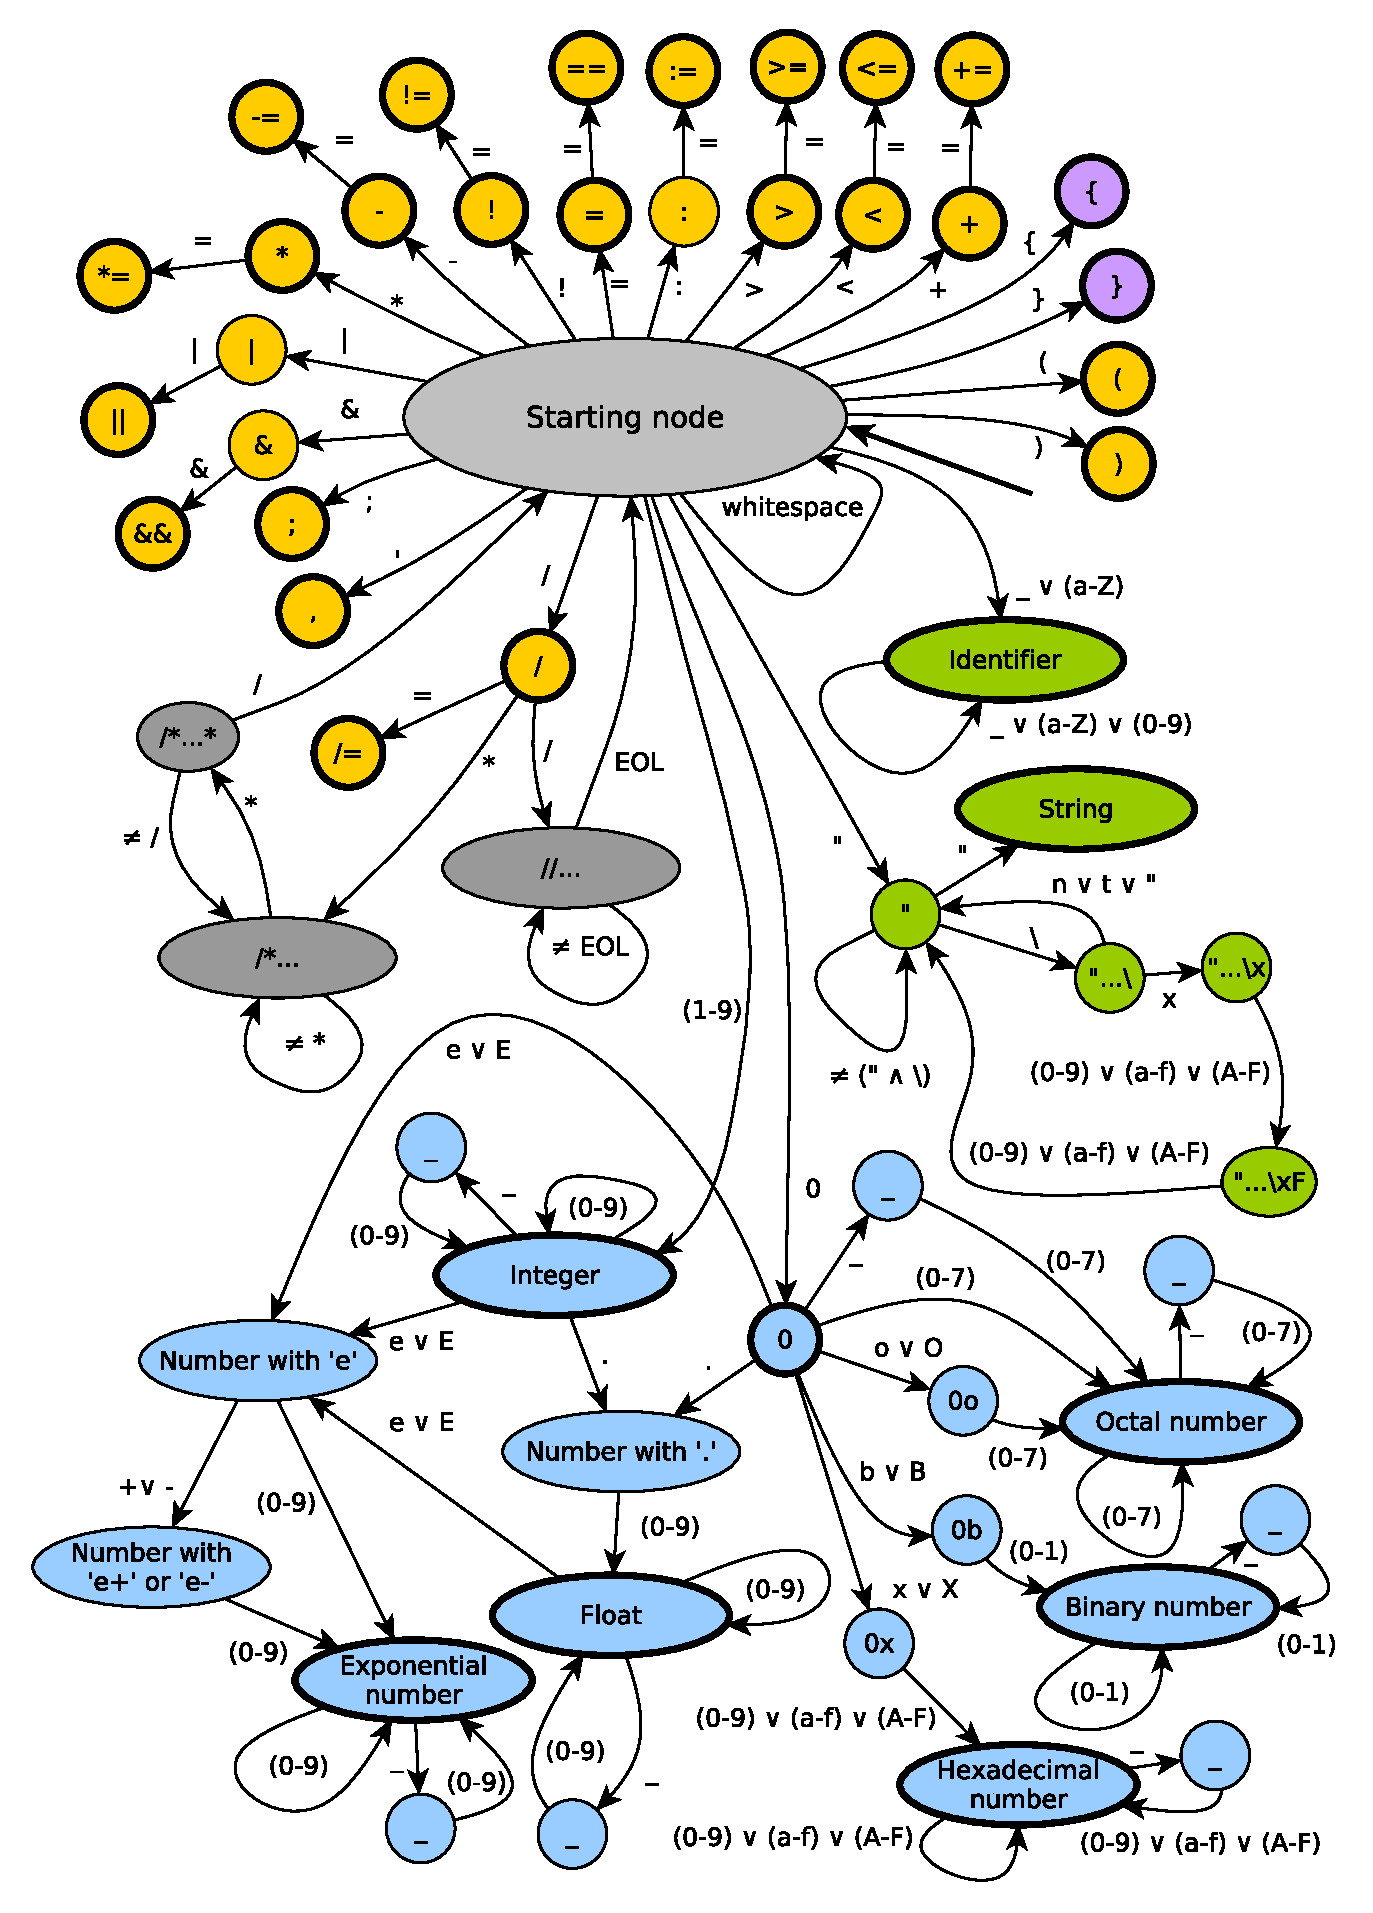
\includegraphics[width=\textwidth, height=22cm]{img/scanner_FA.pdf}\par\vspace{1cm}
    \newpage
    
\subsection{LL gramatika pro rekurzivní sestup}
\begin{tabular} { @{\makebox[2em][c]{\rownumber.}} r !{$\longrightarrow$} l }
    <program> & package id <execution> \\
    <execution> & \epsilon \\
    <execution> & func id ( <params> \ ) <ret\_type> \ \{  <body> \ \} <execution> \\
    <params> & \epsilon \\
    <params> & id <type> <params\_n> \\
    <params\_n> & \epsilon \\
    <params\_n> & , id <type> <params\_n> \\
    <ret\_type> & \epsilon \\
    <ret\_type> & <type> \\
    <ret\_type> & ( <ret\_type\_inner> ) \\
    <ret\_type\_inner> & <params> \\
    <ret\_type\_inner> & <type> <ret\_type\_n> \\
    <ret\_type\_n> & \epsilon \\
    <ret\_type\_n> & , <type> <ret\_type\_n> \\
    <type> & float64 \\
    <type> & int \\
    <type> & string \\
    <type> & bool \\
    <body> & \epsilon \\
    <body> & <statement> <body> \\
    <statement> & expression \\
    <statement> & return <return\_follow> \\
    <statement> & if expression \{ <body> \} <else> \\
    <statement> & for <for\_definition> ; expression ; <for\_assignment> \{ <body> \} \\
    <return\_follow> & \epsilon \\
    <return\_follow> & expression \\
    <else> & \epsilon \\
    <else> & else <else\_n> \\
    <else\_n> & \{ <body> \} \\
    <else\_n> & if expression \{ <body> \} <else> \\
    <for\_definition> & \epsilon \\
    <for\_definition> & expression \\
    <for\_assignment> & \epsilon \\
    <for\_assignment> & expression \\
\end{tabular}
\clearpage


\begin{landscape}
\thispagestyle{empty}
\subsection{LL tabulka}
\label{sec:ll-tab}
\vfill
\begin{tabular}{ |c||c|c|c|c|c|c|c|c|c|c|c|c|c|c|c|c|c|c|c| } \hline
     & package & id & func & ( & ) & \{ & \} & , & float64 & int & string & bool & expression & return & if & for & ; & else & \$ \\ \hline \hline
    <program>&1&&&&&&&&&&&&&&&&&& \\ \hline
    <execution>&&&3&&&&&&&&&&&&&&&&2 \\ \hline
    <params>&&5&&&4&&&&&&&&&&&&&& \\ \hline
    <params\_n>&&&&&6&&&7&&&&&&&&&&& \\ \hline
    <ret\_type>&&&&10&&8&&&9&9&9&9&&&&&&& \\ \hline
    <ret\_type\_inner>&&11&&&11&&&&12&12&12&12&&&&&&& \\ \hline
    <ret\_type\_n>&&&&&13&&&14&&&&&&&&&&& \\ \hline
    <type>&&&&&&&&&15&16&17&18&&&&&&& \\ \hline
    <body>&&&&&&&19&&&&&&20&20&20&20&&& \\ \hline
    <statement>&&&&&&&&&&&&&21&22&23&24&&& \\ \hline
    <return\_follow>&&&&&&&25&&&&&&25, 26&25&25&25&&& \\ \hline
    <else>&&&&&&&27&&&&&&27&27&27&27&&28& \\ \hline
    <else\_n>&&&&&&29&&&&&&&&&30&&&& \\ \hline
    <for\_definition>&&&&&&&&&&&&&32&&&&31&& \\ \hline
    <for\_assignment>&&&&&&33&&&&&&&34&&&&&& \\ \hline
\end{tabular}

\vfill
\raisebox{0.1cm}{\makebox[\linewidth]{\thepage}}
\end{landscape}


\newpage

\subsection{Gramatika pro precedenční analýzu}
\begin{tabular} { @{\makebox[2em][c]{\rownumber.}} r !{$\longrightarrow$} l }
E & ! E \\
E & + E \\
E & - E \\
E & E * E \\
E & E / E \\
E & E + E \\
E & E - E \\
E & E < E \\
E & E > E \\
E & E <= E \\
E & E >= E \\
E & E == E \\
E & E != E \\
E & E \&\& E \\
E & E || E \\
E & E = E \\
E & E, \ldots \hspace{1pt} = E \\
E & E, \ldots \hspace{1pt} = E, \ldots \\
E & E := E \\
E & E, \ldots \hspace{1pt} = E \\
E & E, \ldots \hspace{1pt} = E, \ldots \\
E & E += E \\
E & E -= E \\
E & E *= E \\
E & E /= E \\
E & (E) \\
E & i \\
E & f() \\
E & f(E) \\ 
E & f(E, \ldots) \\
\end{tabular}
\newpage

\begin{landscape}
\thispagestyle{empty}

\subsection{Precedenční tabulka}
\begin{tabular}{ |c||c|c|c|c|c|c|c|c|c|c|c|c|c|c|c|c|c|c|c|c|c|c|c|c|c|c|c| } \hline
     & ! & + (U) & - (U) & * & / & + & - & < & > & <= & >= & == & != & \&\& & || & = & := & += & -= & *= & /= & ( & ) & i & f & , & \$ \\ \hline \hline
     ! &<&<&<&>&>&>&>&>&>&>&>&>&>&>&>&&&&&&&<&>&<&<&>&> \\ \hline
     + (U) &<&<&<&>&>&>&>&>&>&>&>&>&>&>&>&&&&&&&<&>&<&<&>&> \\ \hline
     - (U) &<&<&<&>&>&>&>&>&>&>&>&>&>&>&>&&&&&&&<&>&<&<&>&> \\ \hline
     * &<&<&<&>&>&>&>&>&>&>&>&>&>&>&>&&&&&&&<&>&<&<&>&> \\ \hline
     / &<&<&<&>&>&>&>&>&>&>&>&>&>&>&>&&&&&&&<&>&<&<&>&> \\ \hline
     + &<&<&<&<&<&>&>&>&>&>&>&>&>&>&>&&&&&&&<&>&<&<&>&> \\ \hline
     - &<&<&<&<&<&>&>&>&>&>&>&>&>&>&>&&&&&&&<&>&<&<&>&> \\ \hline
     < &<&<&<&<&<&<&<&>&>&>&>&>&>&>&>&&&&&&&<&>&<&<&>&> \\ \hline
     > &<&<&<&<&<&<&<&>&>&>&>&>&>&>&>&&&&&&&<&>&<&<&>&> \\ \hline
     <= &<&<&<&<&<&<&<&>&>&>&>&>&>&>&>&&&&&&&<&>&<&<&>&> \\ \hline
     >= &<&<&<&<&<&<&<&>&>&>&>&>&>&>&>&&&&&&&<&>&<&<&>&> \\ \hline
     == &<&<&<&<&<&<&<&>&>&>&>&>&>&>&>&&&&&&&<&>&<&<&>&> \\ \hline
     != &<&<&<&<&<&<&<&>&>&>&>&>&>&>&>&&&&&&&<&>&<&<&>&> \\ \hline
     \&\& &<&<&<&<&<&<&<&<&<&<&<&<&<&>&>&&&&&&&<&>&<&<&>&> \\ \hline
    || &<&<&<&<&<&<&<&<&<&<&<&<&<&<&>&&&&&&&<&>&<&<&>&> \\ \hline
     = &<&<&<&<&<&<&<&<&<&<&<&<&<&<&<&&&&&&&<&&<&<&=&> \\ \hline
    := &<&<&<&<&<&<&<&<&<&<&<&<&<&<&<&&&&&&&<&&<&<&=&> \\ \hline
    += &<&<&<&<&<&<&<&<&<&<&<&<&<&<&<&&&&&&&<&&<&<&&> \\ \hline
    -= &<&<&<&<&<&<&<&<&<&<&<&<&<&<&<&&&&&&&<&&<&<&&> \\ \hline
    *= &<&<&<&<&<&<&<&<&<&<&<&<&<&<&<&&&&&&&<&&<&<&&> \\ \hline
    /= &<&<&<&<&<&<&<&<&<&<&<&<&<&<&<&&&&&&&<&&<&<&&> \\ \hline
     ( &<&<&<&<&<&<&<&<&<&<&<&<&<&<&<&&&&&&&<&=&<&<&=& \\ \hline
     ) &>&>&>&>&>&>&>&>&>&>&>&>&>&>&>&&&&&&&&>&&&>&> \\ \hline
     i &>&>&>&>&>&>&>&>&>&>&>&>&>&>&>&>&>&>&>&>&>&&>&&&>&> \\ \hline
     f &&&&&&&&&&&&&&&&&&&&&&=&&&&& \\ \hline
     , &<&<&<&<&<&<&<&<&<&<&<&<&<&<&<&=&=&&&&&<&=&<&<&=&> \\ \hline
     \$ &<&<&<&<&<&<&<&<&<&<&<&<&<&<&<&<&<&<&<&<&<&<&&<&<&<& \\ \hline
     
\end{tabular}
\vfill
\raisebox{0.1cm}{\makebox[\linewidth]{\thepage}}
\end{landscape}



\end{document}